\chapter{Table recognition implementation}

This chapter gives us an overview of procedures and tools used to create a table recognition software. 

The project is written in C++ and compilable using CMake (tested on \\MSVC~2017 and g++~7.4). We chose CMake for its cross-platform support and its ability to work with external dependencies (e.g. Tesseract, Leptonica). 

The implementation is divided into two main parts --- \emph{preprocessing}, which prepares the input images for recognition, and \emph{tabular OCR}, which applies our heuristic algorithm for table recognition. Both parts use the features of the Leptonica library and tabular OCR utilizes the character and textline recognition of the Tesseract engine. The image processing in the program is schematized in~\cref{fig:programFlow}.

\begin{figure}
    \centering
	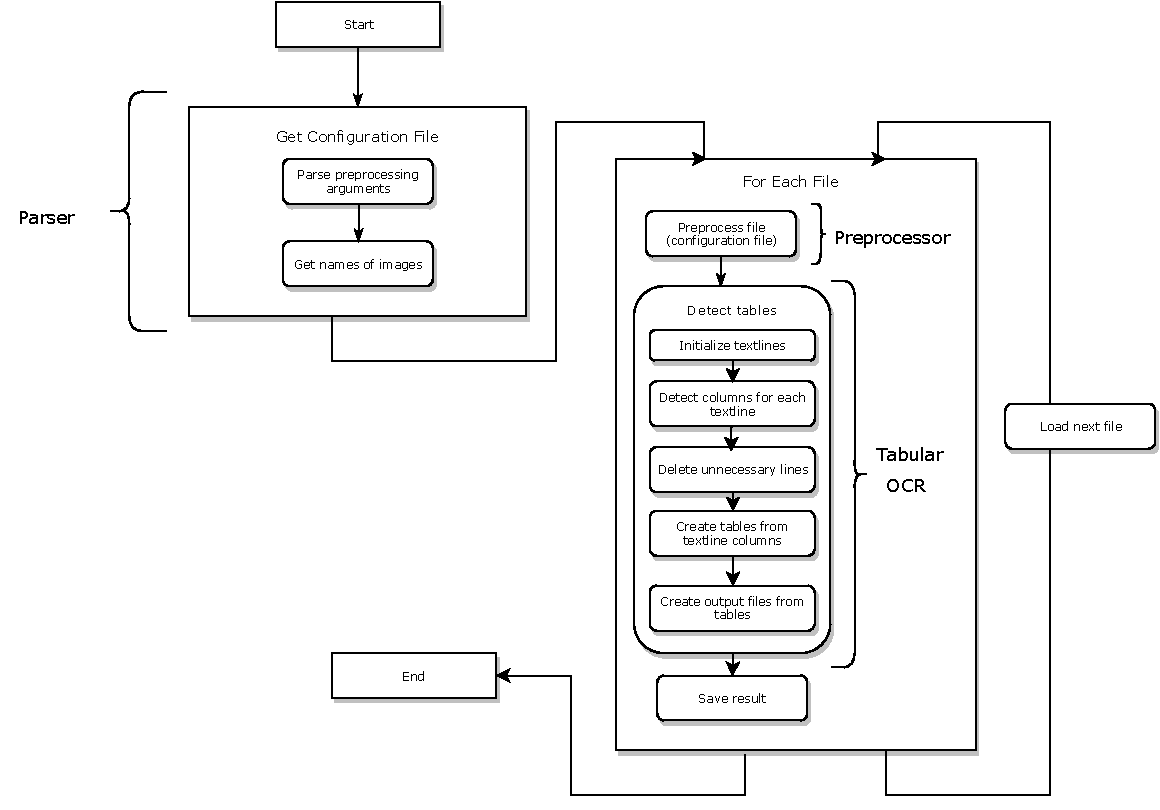
\includegraphics[width=1.0\linewidth]{img/implementation/programFlow.pdf}
	\caption{Program flow diagram.}
	\label{fig:programFlow}
\end{figure}

\section{Preprocessing}

The preprocessing part is basically a wrapper around the Leptonica library. Based on the input arguments of our software, the preprocessor calls relevant Leptonica's methods with specified parameters. Not all of the Leptonica's preprocessing features are currently supported in our implementation. However, it is a simple task to add the rest of them. Currently supported methods are the following:

\begin{itemize}
    \item \emph{Contrast enhancement}, specifically histogram equalization (see~\cref{contrastEnhancemet}), a method of non-linear stretching called gamma correction~\cite{rahman2016adaptive}, and a simple method of linear stretching based on an arctangent function.
    \item \emph{Greyscale conversion}, specifically the averaging technique and luma correction technique (both mentioned in~\cref{grayscaleConversion}). Supported are also two techniques from the Leptonica library based on the selection of either the maximal or minimal value from the three RGB components.
    \item \emph{Binarization}, specifically the support of Otsu and Sauvola binarization techniques (see~\cref{binarization}).
    \item \emph{Deskewing}, which does not contain any options. This is due to the fact that Leptonica contains only one deskewing function, which is based on the calculation of projection profiles (see~\cref{deskewing}) with the help of Hough transform~\cite{bloomberg2analysis}.
\end{itemize}

The initial idea for preprocessing was to provide more complex functions which are included in the OpenCV library~\cite{OpenCV}. However, this was not the goal of the thesis. Therefore, the preprocessing part stayed very simple and mostly demonstrative and the user is still advised to preprocess the images manually.

\section{Tabular OCR}

After the preprocessing part is done, the preprocessed image is passed to tabular OCR for table recognition. The individual steps of our heuristic table recognition algorithm are executed in the main \texttt{process\_image} function.

In this section, we analyze this algorithm step-by-step and overview the functions used. During the process, we use the concept of \emph{textlines} --- rows of the image document that contain recognized character symbols.

Our algorithm is based on the already mentioned Tesseract symbol and textline recognition (see~\cref{tesseractCharacterRecognition}) and moreover on whitespace detection. Upon detecting whitespaces between individual symbols, we try to heuristically estimate the whitespaces between words and, furthermore, columns, for each textline of the image. Once we have all the textlines separated into columns, we try to merge consecutive lines with similar column layout into a table.  

Following are the individual steps of the algorithm, also visualized in~\cref{fig:implemTableRecogniton}:
\begin{enumerate}
\item \emph{Textline initialization}, which includes the Tesseract recognition process, and from its output obtains all the required information about individual textlines.
\item \emph{Deletion of unnecessary lines}, which removes textlines with no valuable information (e.g. textlines with no symbols, false positives).
\item \emph{Column detection}, which determines the column segmentation for each existing textline.
\item \emph{Column merge into tables}, which merges the existing textlines into tables based on their column layout.
\item \emph{Output determination}, which processes the information in each recognized table and outputs it in a meaningful structure.
\end{enumerate}

\subsection{Textline initialization} \label{textlineInitialization}

The whole process begins with the detection of individual characters and their merge into textlines (\cref{fig:implem1}).

For the purposes of the character recognition, we use the Tesseract engine. We initialize the Tesseract API without the use of neural networks and obtain both lines and symbols. We decided to not use the neural networks due to the fact that they did not produce as accurate results as simple heuristic recognition at the time of testing. However, their performance may increase over the time. Therefore, this setting might need to be manually changed in the future.

After this step, we do not use the features of the Tesseract engine anymore, and rely solely on our heuristic functions.

The symbols and lines obtained from Tesseract are represented as simple boxes, with the symbols also containing textual information. To gain a more detailed information about individual textlines, we therefore iterate over all the lines and symbols and assign symbols into their lines. The result of this function is therefore a list of all textlines containing the information about their individual symbols, like positioning and their actual character value in UTF8.

This function runs in $O(m\cdot n^2)$. The initial idea for this implementation was to firstly sort both the symbols and lines by their y coordinates (which is simply $O(\log n)$ and $O(\log m)$). The assignment of individual symbols into their lines would then be performed by simply iterating symbols and jumping to another line once the current symbol does not fit in the current line, with the iteration therefore having a $O(m\cdot n)$ time complexity. This would present a significant execution time improvement.

However, a problem occurred with this approach. By default, Tesseract's recognition creates a lot of false positives, including noise recognized as dots, white spaces, and, most importantly, horizontal and vertical lines, like footer or header separators, underlinings of words, table borders, etc. These false positives disrupt the reading order of the document, which is a factor that this approach relies on.

Although we tried to remove these false positives (for example, removal of empty characters was trivial and required only checking for symbols that contain no textual information), we found no criterion that would suffice all of these obstacles. Therefore, in our current approach, we chose to sacrifice time complexity in favor of accuracy.

\subsection{Deletion of unnecessary lines}

As already mentioned, Tesseract's textline recognition algorithm may include false positives. In this step, we delete all unnecessary lines (\cref{fig:implem2}), specifically:

\begin{itemize}
\item \emph{Empty lines}

Like horizontal and vertical line segments, borders or other lines that contain no UTF8 symbols are of no use and are therefore removed from the textline list.

\item \emph{Table textlines}

Table textlines are parts of the image that are bordered by visible lines, which usually represent either a table, form or even a graphics image. Tesseract often recognizes these parts as single textlines. These textlines therefore contain multiple other textlines, and are significantly greater in height. We remove them by a simple heuristic based on the comparison of their height and the font of their symbols.
\end{itemize}

We present both cases of unnecessary lines in~\cref{fig:deletionOfLines}.

Once this step of the algorithm is done, we are left only with lines that contain symbols and can be a part of the table.

\begin{figure}
\centering
{\sffamily
\begin{tabular}{cc}
Empty lines & Table textline \\
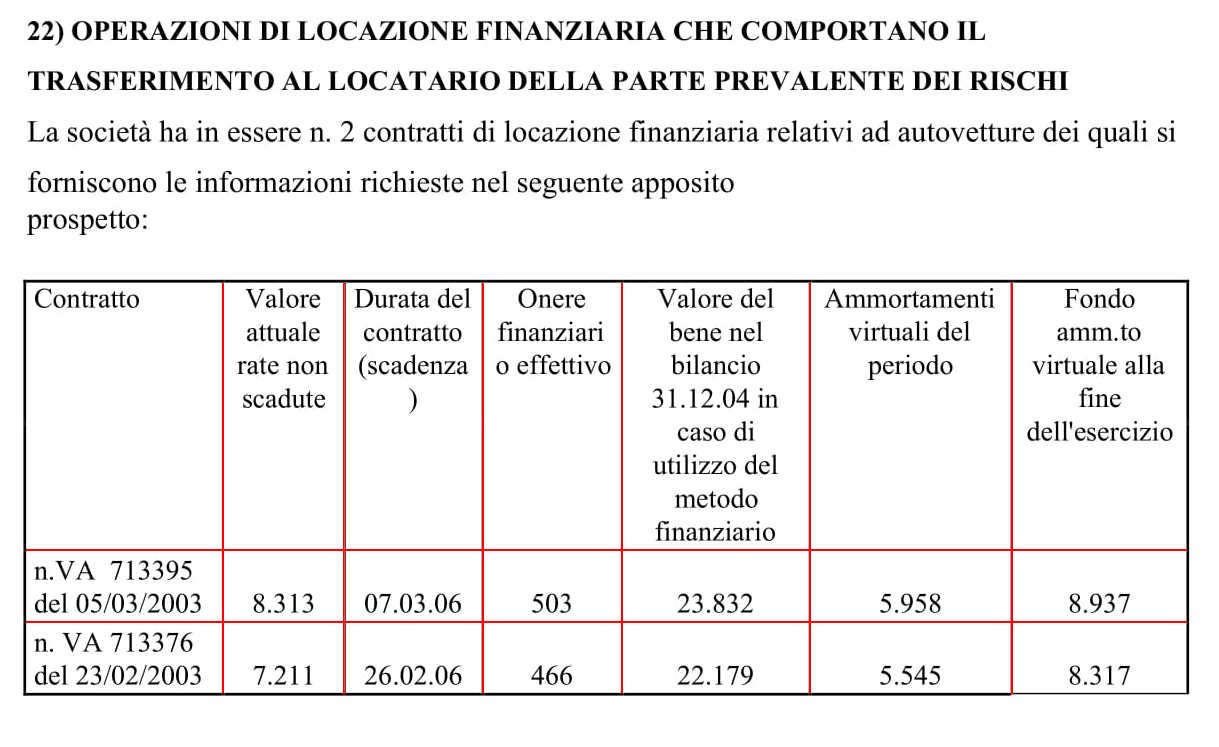
\includegraphics[width=0.4\linewidth]{img/implementation/textlineEmpty.png}
&
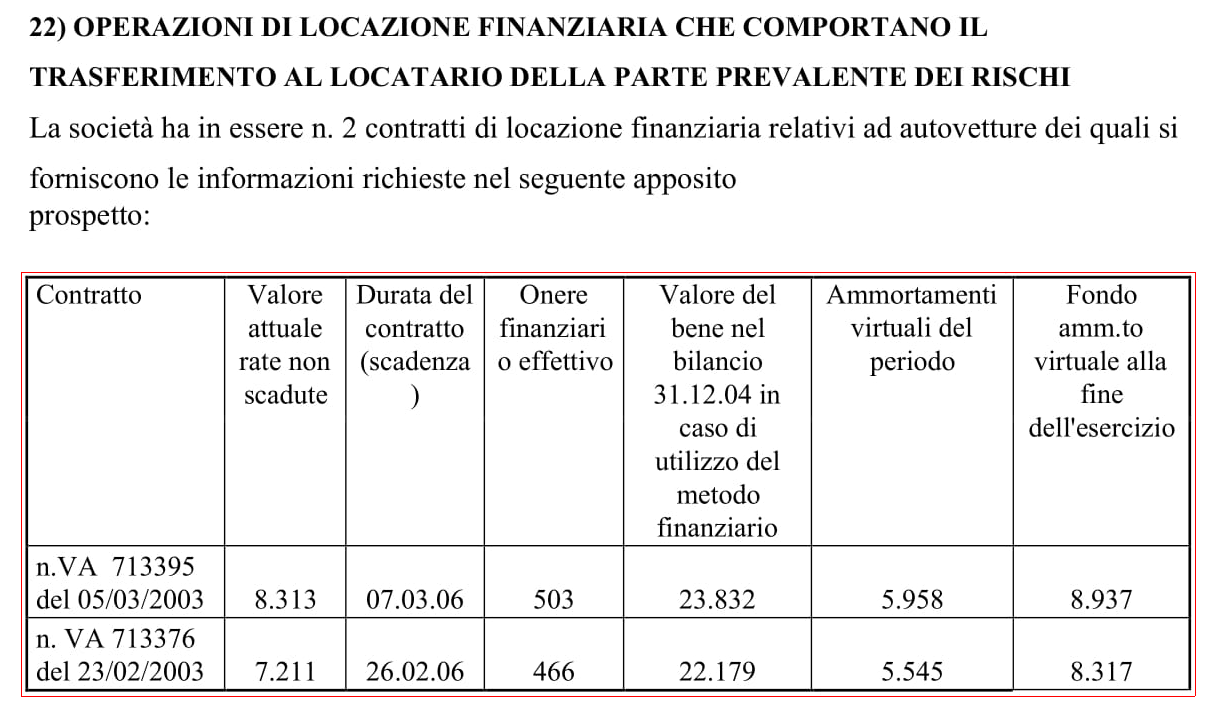
\includegraphics[width=0.4\linewidth]{img/implementation/textlineTable.png}\\
\end{tabular}
}
\caption{Types of unnecessary lines that Tesseract might have recognized as textlines. We remove these lines by heuristic algorithms.}
\label{fig:deletionOfLines}
\end{figure}

\subsection{Column detection} \label{columnDetection}

Upon obtaining individual textlines, we try to determine their segmentation into columns by analyzing the positions of symbols they contain. This is done for each line individually. Symbols are merged into words and then into columns (\cref{fig:implem3}). Although we could simply merge symbols into columns and ignore the whole processing of words, this would leave us with no information about word spaces and would therefore lead to merging of text.

We start this process by obtaining all the spaces between individual symbols and sorting them by size. The resulting list of spaces is then used to determine word space size using a \emph{multiplication factor}. 

Multiplication factor is used to decide whether an element of the sorted space sizes list differs enough from its predecessor to be a word space. From the results of the detection of spaces between individual symbols, we have observed that the greater the current space is, the less the multiplication factor should be. Based on this, we have tried many different values and curves for the determination of the multiplication factor. First observations from these attempts led to the estimation that the best curve to use would be logarithmic. However, the current implementation seemed to worked well enough and was therefore left as it is.

The determination of the column whitespace was based on a similar idea with slightly altered parameters.

Upon determining the column and word whitespaces, we then merge symbols by these whitespaces into words and columns respectively, as shown in~\cref{fig:symbolMerging}.

The determination of whitespaces was probably the most difficult part of the algorithm. There have been multiple different ideas for the implementation. The one that has been preferred most of the time was the idea of separating textlines according to their font sizes. The ones with similar fonts were assigned to the same \emph{font category}, and the whitespace was then determined for the whole category. The word whitespace recognition worked slightly better with this approach. However, the determination of columns had a higher chance of failure, as the sizes of column spaces greatly differ in each line. Therefore, the current simpler approach was chosen.

Another initial idea was to simply determine the size of the column space by a constant, e.g. $word\_whitespace*constant = column\_whitespace$. Surprisingly, the results of this approach were comparable to those of the current implementation. However, it was prone to errors, especially when the input image contained small fonts or full-page tables, and had no room for improvement in contrast to the current approach.

\begin{figure}
\centering
{\sffamily
\begin{tabular}{c}
The original image \\
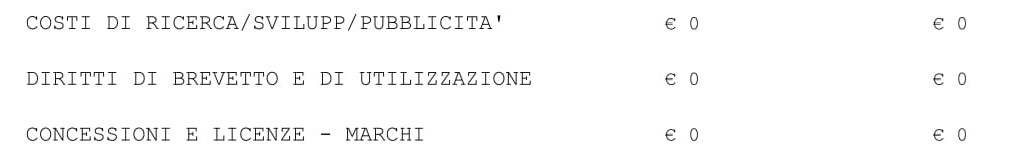
\includegraphics[width=0.8\linewidth]{img/implementation/mergedOrig.jpg}\\
Merged into words \\
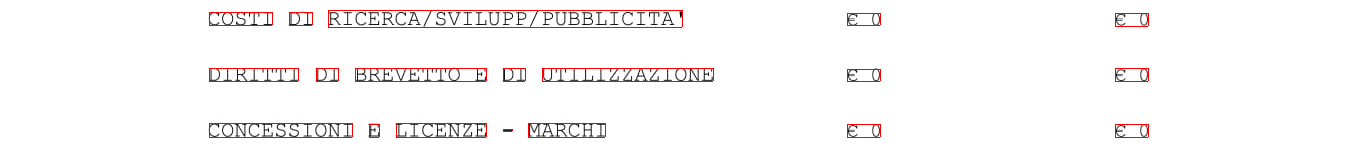
\includegraphics[width=0.8\linewidth]{img/implementation/mergedWords.png}\\
Merged into columns \\
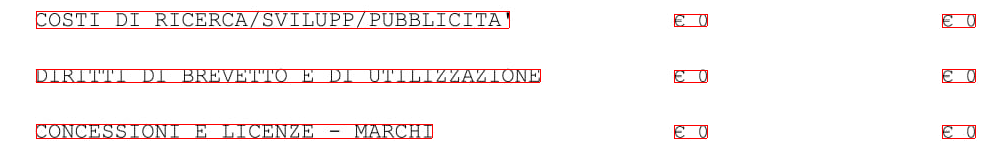
\includegraphics[width=0.8\linewidth]{img/implementation/mergedCols.png}\\
\end{tabular}
}
\caption{The process of merging symbols of a textline.}
\label{fig:symbolMerging}
\end{figure}

\subsection{Column merge into tables}

Once we have the information about columns for each textline, we can start searching for tables. The table detection algorithm is performed by a simple $O(n)$ algorithm by iterating the textlines from top to bottom and merging two consecutive textlines with similar column layout. 

The determination of whether two textlines have similar column layout is performed according to~\cref{alg:tableMerge}.

\begin{algorithm}[t]
\caption{Are textlines in same table}
{\scriptsize
\label{alg:tableMerge}
\begin{algorithmic}
\Require first\_col \Comment represents the current place we are when iterating over columns of first line
\State second\_col \Comment represents the current place we are when iterating over columns of second line
\While{true}
\If {either first\_col or second\_col is at the end of their line}
\If {at least one pair of columns was found that should be merged}
\State \emph{merge}
\Else
\State create a table if there are any merged lines
\EndIf
\State \emph{break}
\EndIf
\If {current columns do not overlap}
\If {first\_col has lower x-axis than second\_col}
\State first\_col = first\_col + 1 
\Else
\State second\_col = second\_col + 1 
\EndIf
\State \emph{continue}
\EndIf
\If {found columns do not overlap with other existing columns}
\State save the position of overlapping columns for future merging
\Else
\State create a table if there are any merged lines
\EndIf
\State first\_col = first\_col + 1 
\State  second\_col = second\_col + 1 
\EndWhile
\end{algorithmic}}
\end{algorithm}

From the recognized tables represented by textlines, we create cells by simply overlaying rows and columns and saving their common areas. The problem arises with the existence of multi-line rows, that is, rows that often span over multiple textlines. In our implementation, a simple constant-based algorithm is added to recognize at least some of them and therefore merge multiple textlines into one row.

\subsection{Output determination}

Once we obtain the individual cells, the only thing left is to create a user-friendly representation of the recognized data. Here, the user has two options according to the parameter he sets in the command line environment. 

The first option is a simple image output. Recognized cells are bordered by colored boxes (\cref{fig:implem4}) in the original input image and saved in a PNG file.

The other option is a JSON structure of the recognized cells, which also contains text within each cell. The JSON structure is demonstrated in~\cref{fig:jsonout}.

\begin{figure}[t]
\lstset{
    string=[s]{"}{"},
    stringstyle=\color{blue},
    comment=[l]{:},
    commentstyle=\color{black},
    basicstyle=\scriptsize
}
\begin{lstlisting}
{"all_tables": {
  "cols": number of columns,
  "rows": number of rows,
  "table_repres": {
    "h": height of table,
    "w": width of table,
    "x": the x-coordinate where the table starts,
    "y": the y-coordinate where the table starts
  },
  "cells": [
        {
        "box": {
           "h": height of current cell,
           "w": width of current cell,
           "x": the x-coordinate where the cell starts,
           "y": they y-coordinate where the cells starts
        },
        "cols_no": in which column of the table the cell is,
        "rows_no": in which row of the table the cell is,
        "text": the UTF8 text displayed in the cell
        },
        ...
        other cells
    ]
  }
  ...
  other tables
}
\end{lstlisting}
\caption{A JSON structure used for the representation of tables recognized from an input image.}
\label{fig:jsonout}
\end{figure}

By default, both output options are selected and therefore two files are saved in the newly created \emph{results} directory next to the executable.

\begin{figure}[p]
\begin{subfigure}{0.45\textwidth}
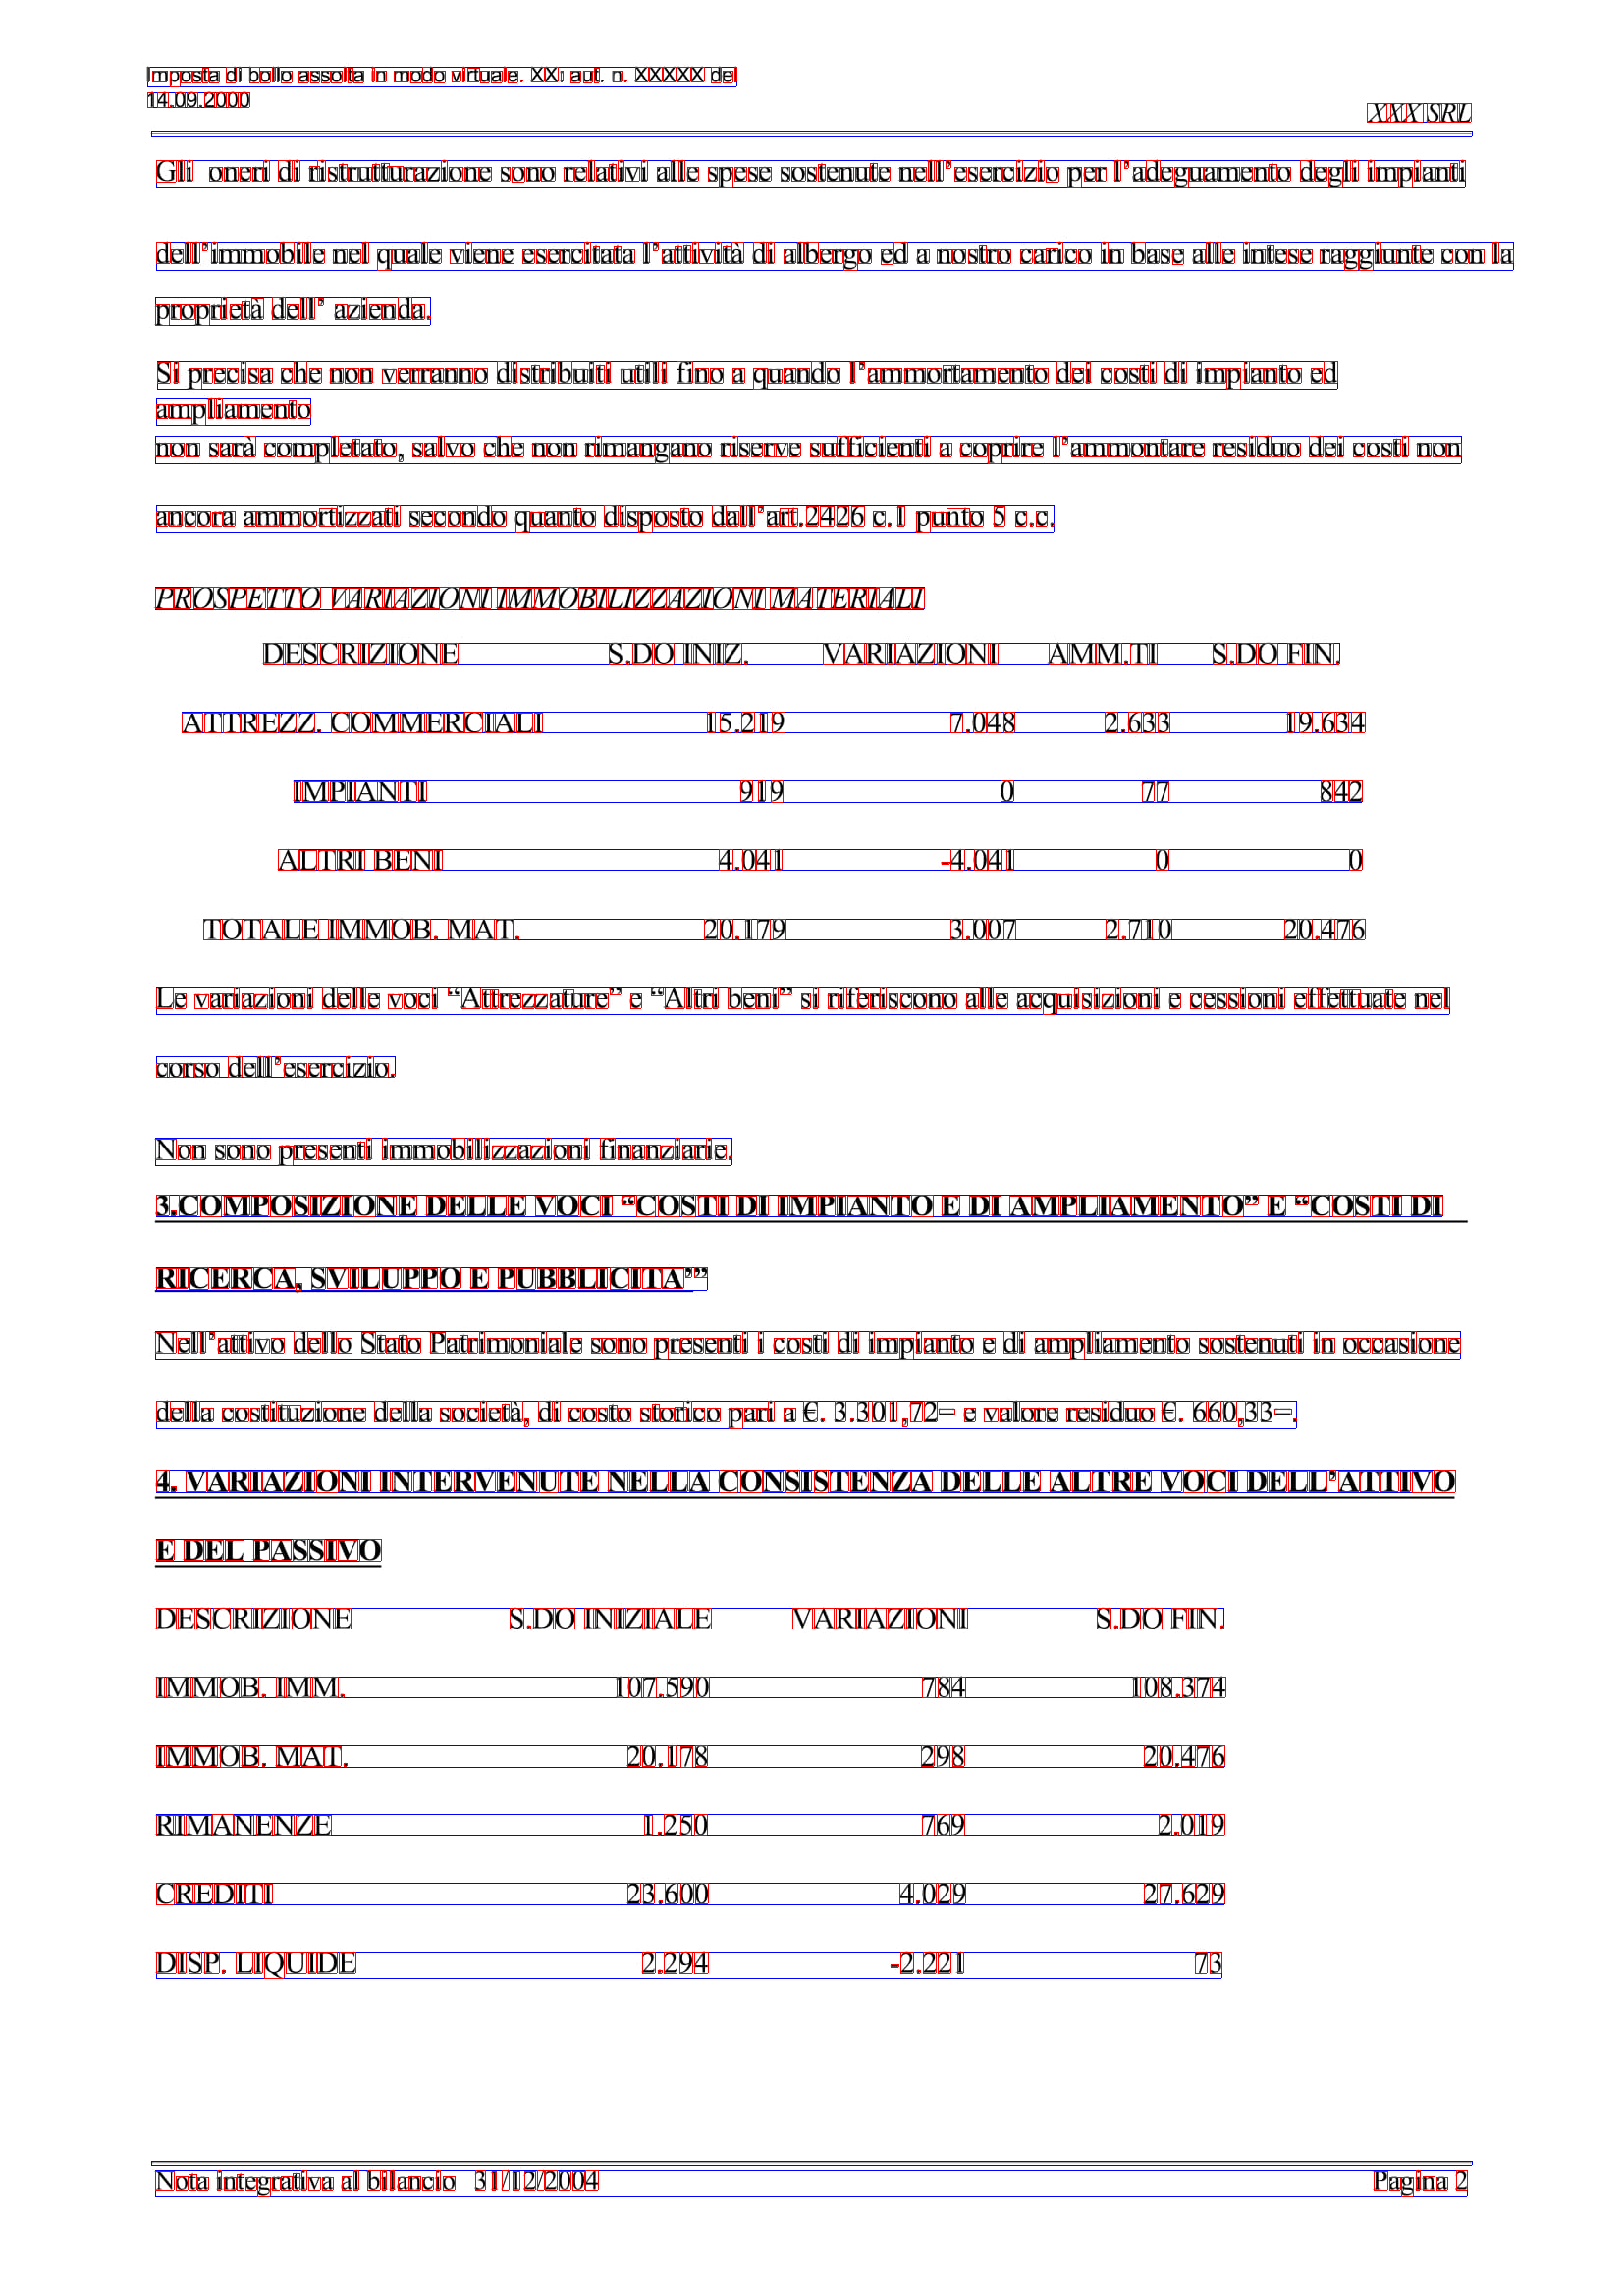
\includegraphics[width=\linewidth]{img/implementation/implem1.png}
\caption{Recognized textlines (blue) and their symbols (red) by the Tesseract recognition. These are merged so the symbols are assigned to their textlines.}
\label{fig:implem1}
\end{subfigure}
\qquad
\begin{subfigure}{0.45\textwidth}
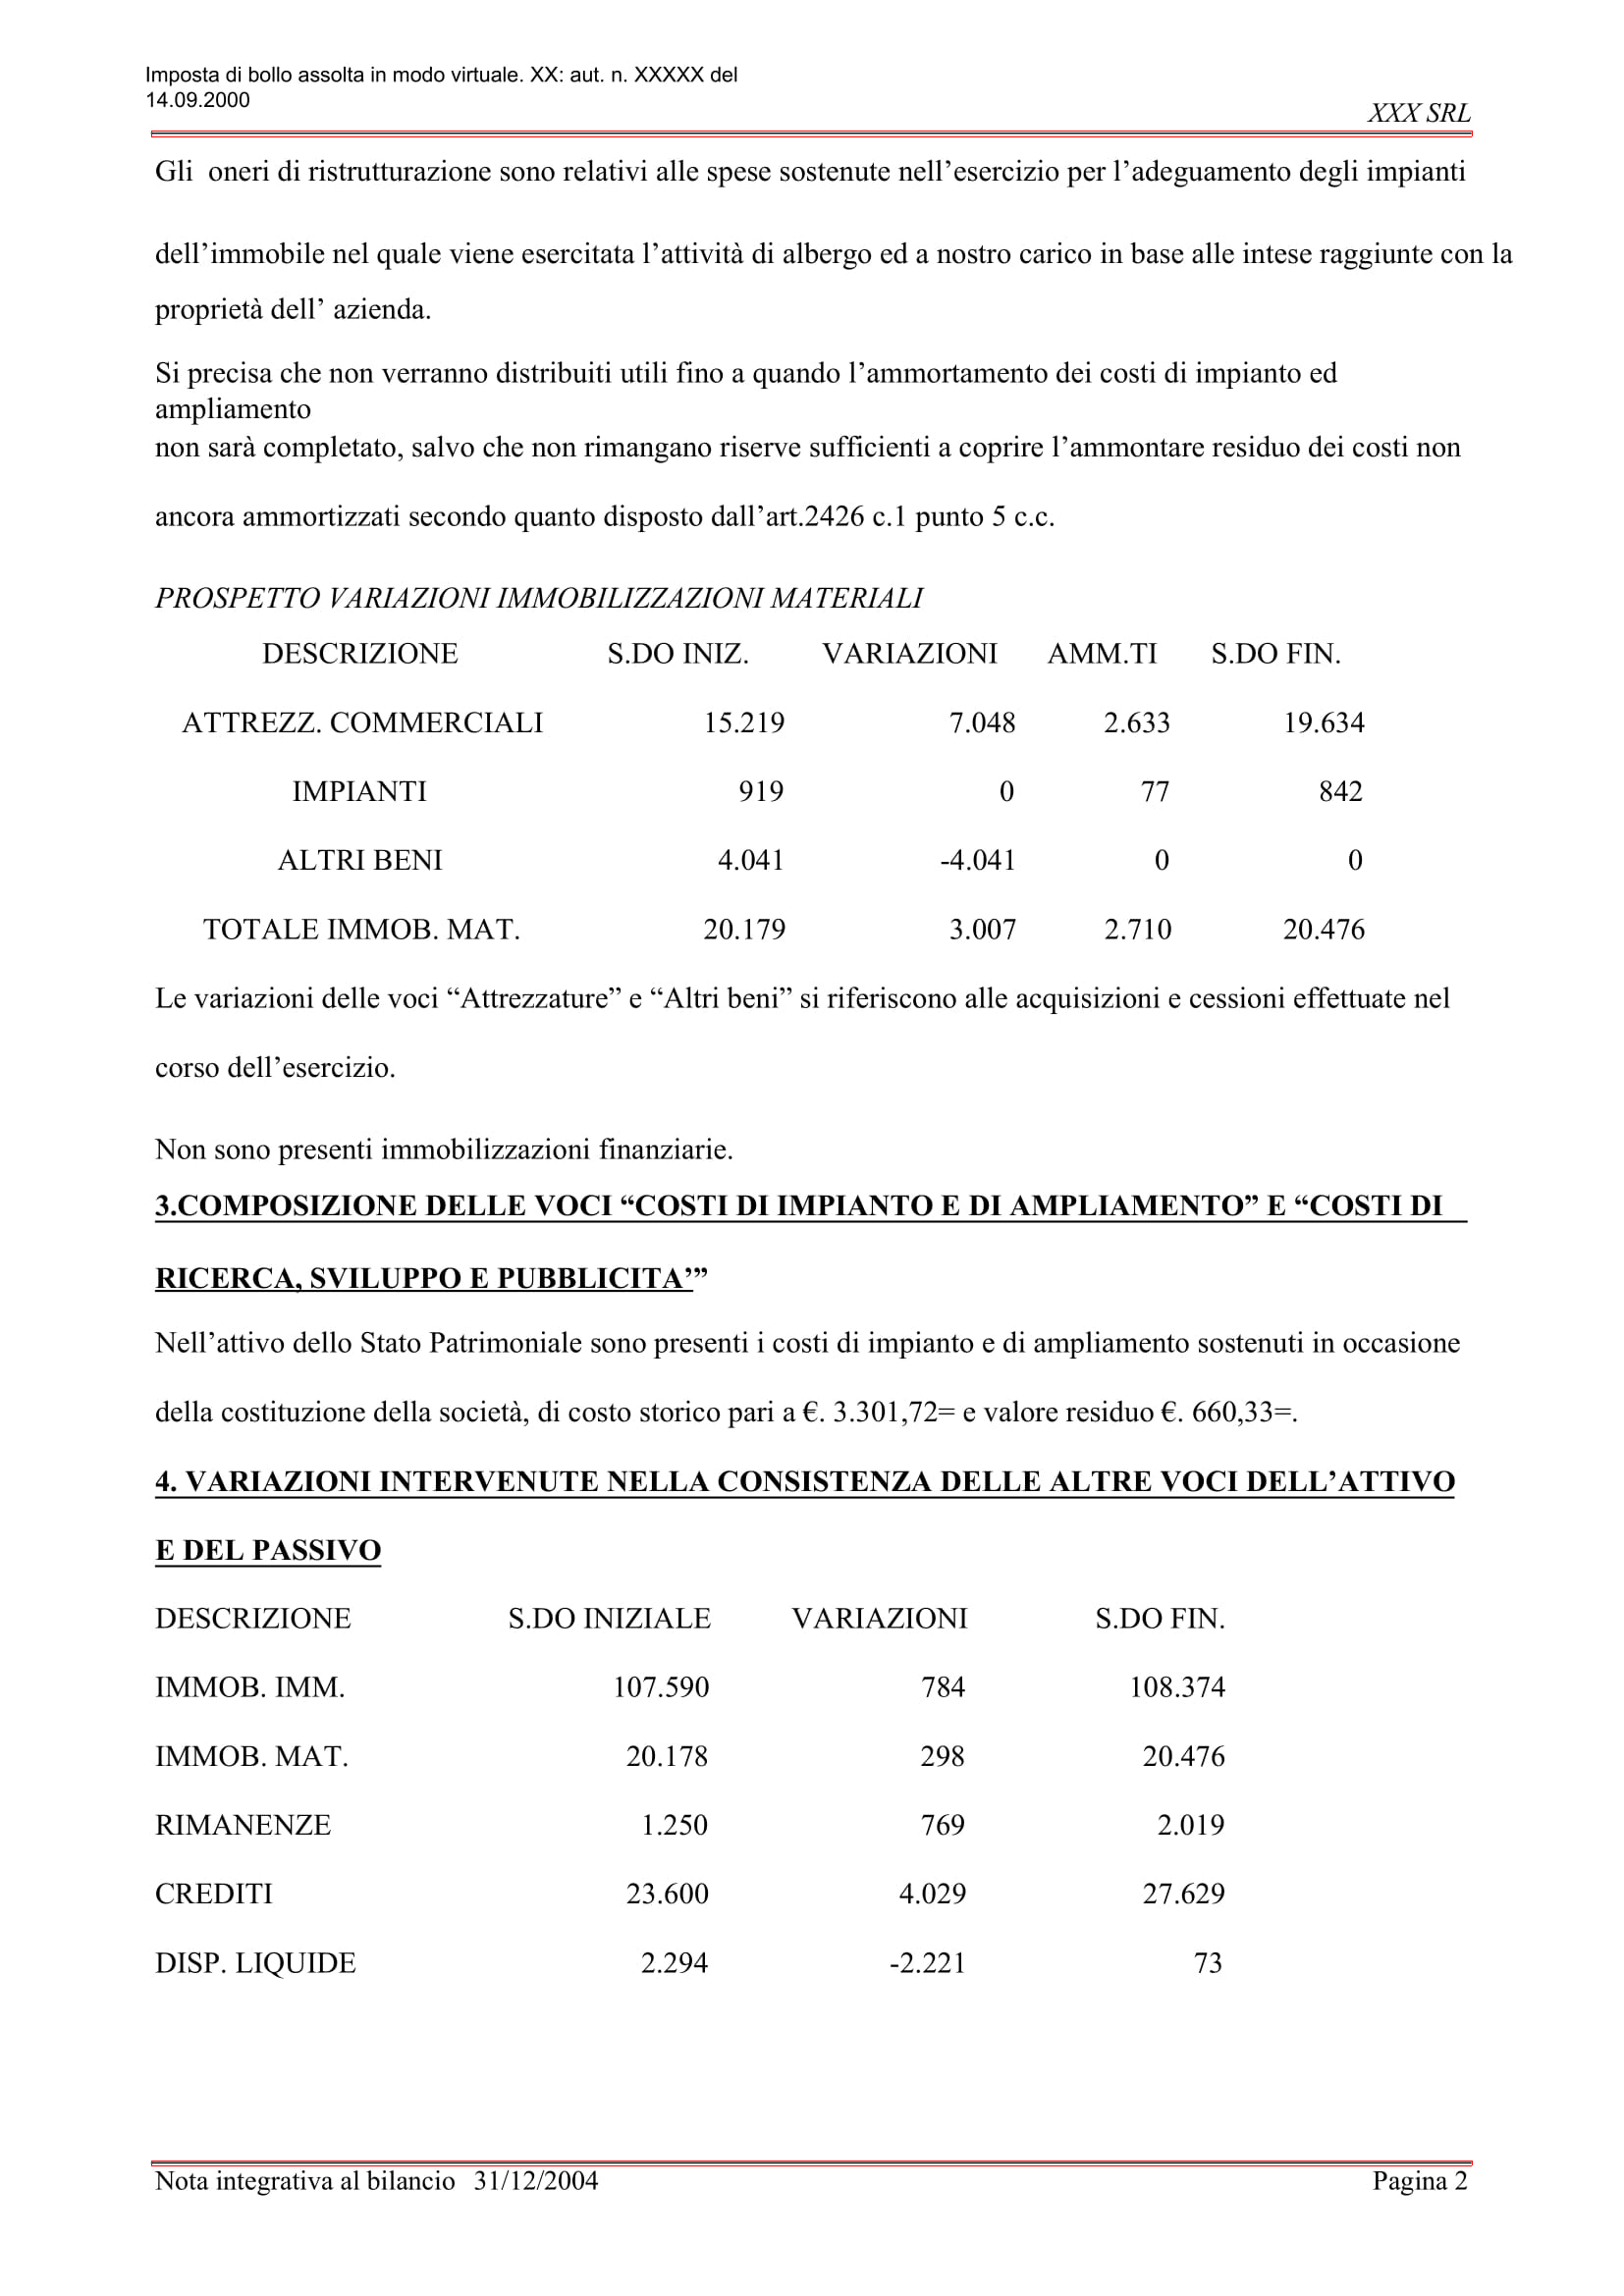
\includegraphics[width=\linewidth]{img/implementation/implem2.png}
\caption{Unnecessary lines recognized from the image. These are removed during the algorithm.}
\label{fig:implem2}
\end{subfigure}
\begin{subfigure}{0.45\textwidth}
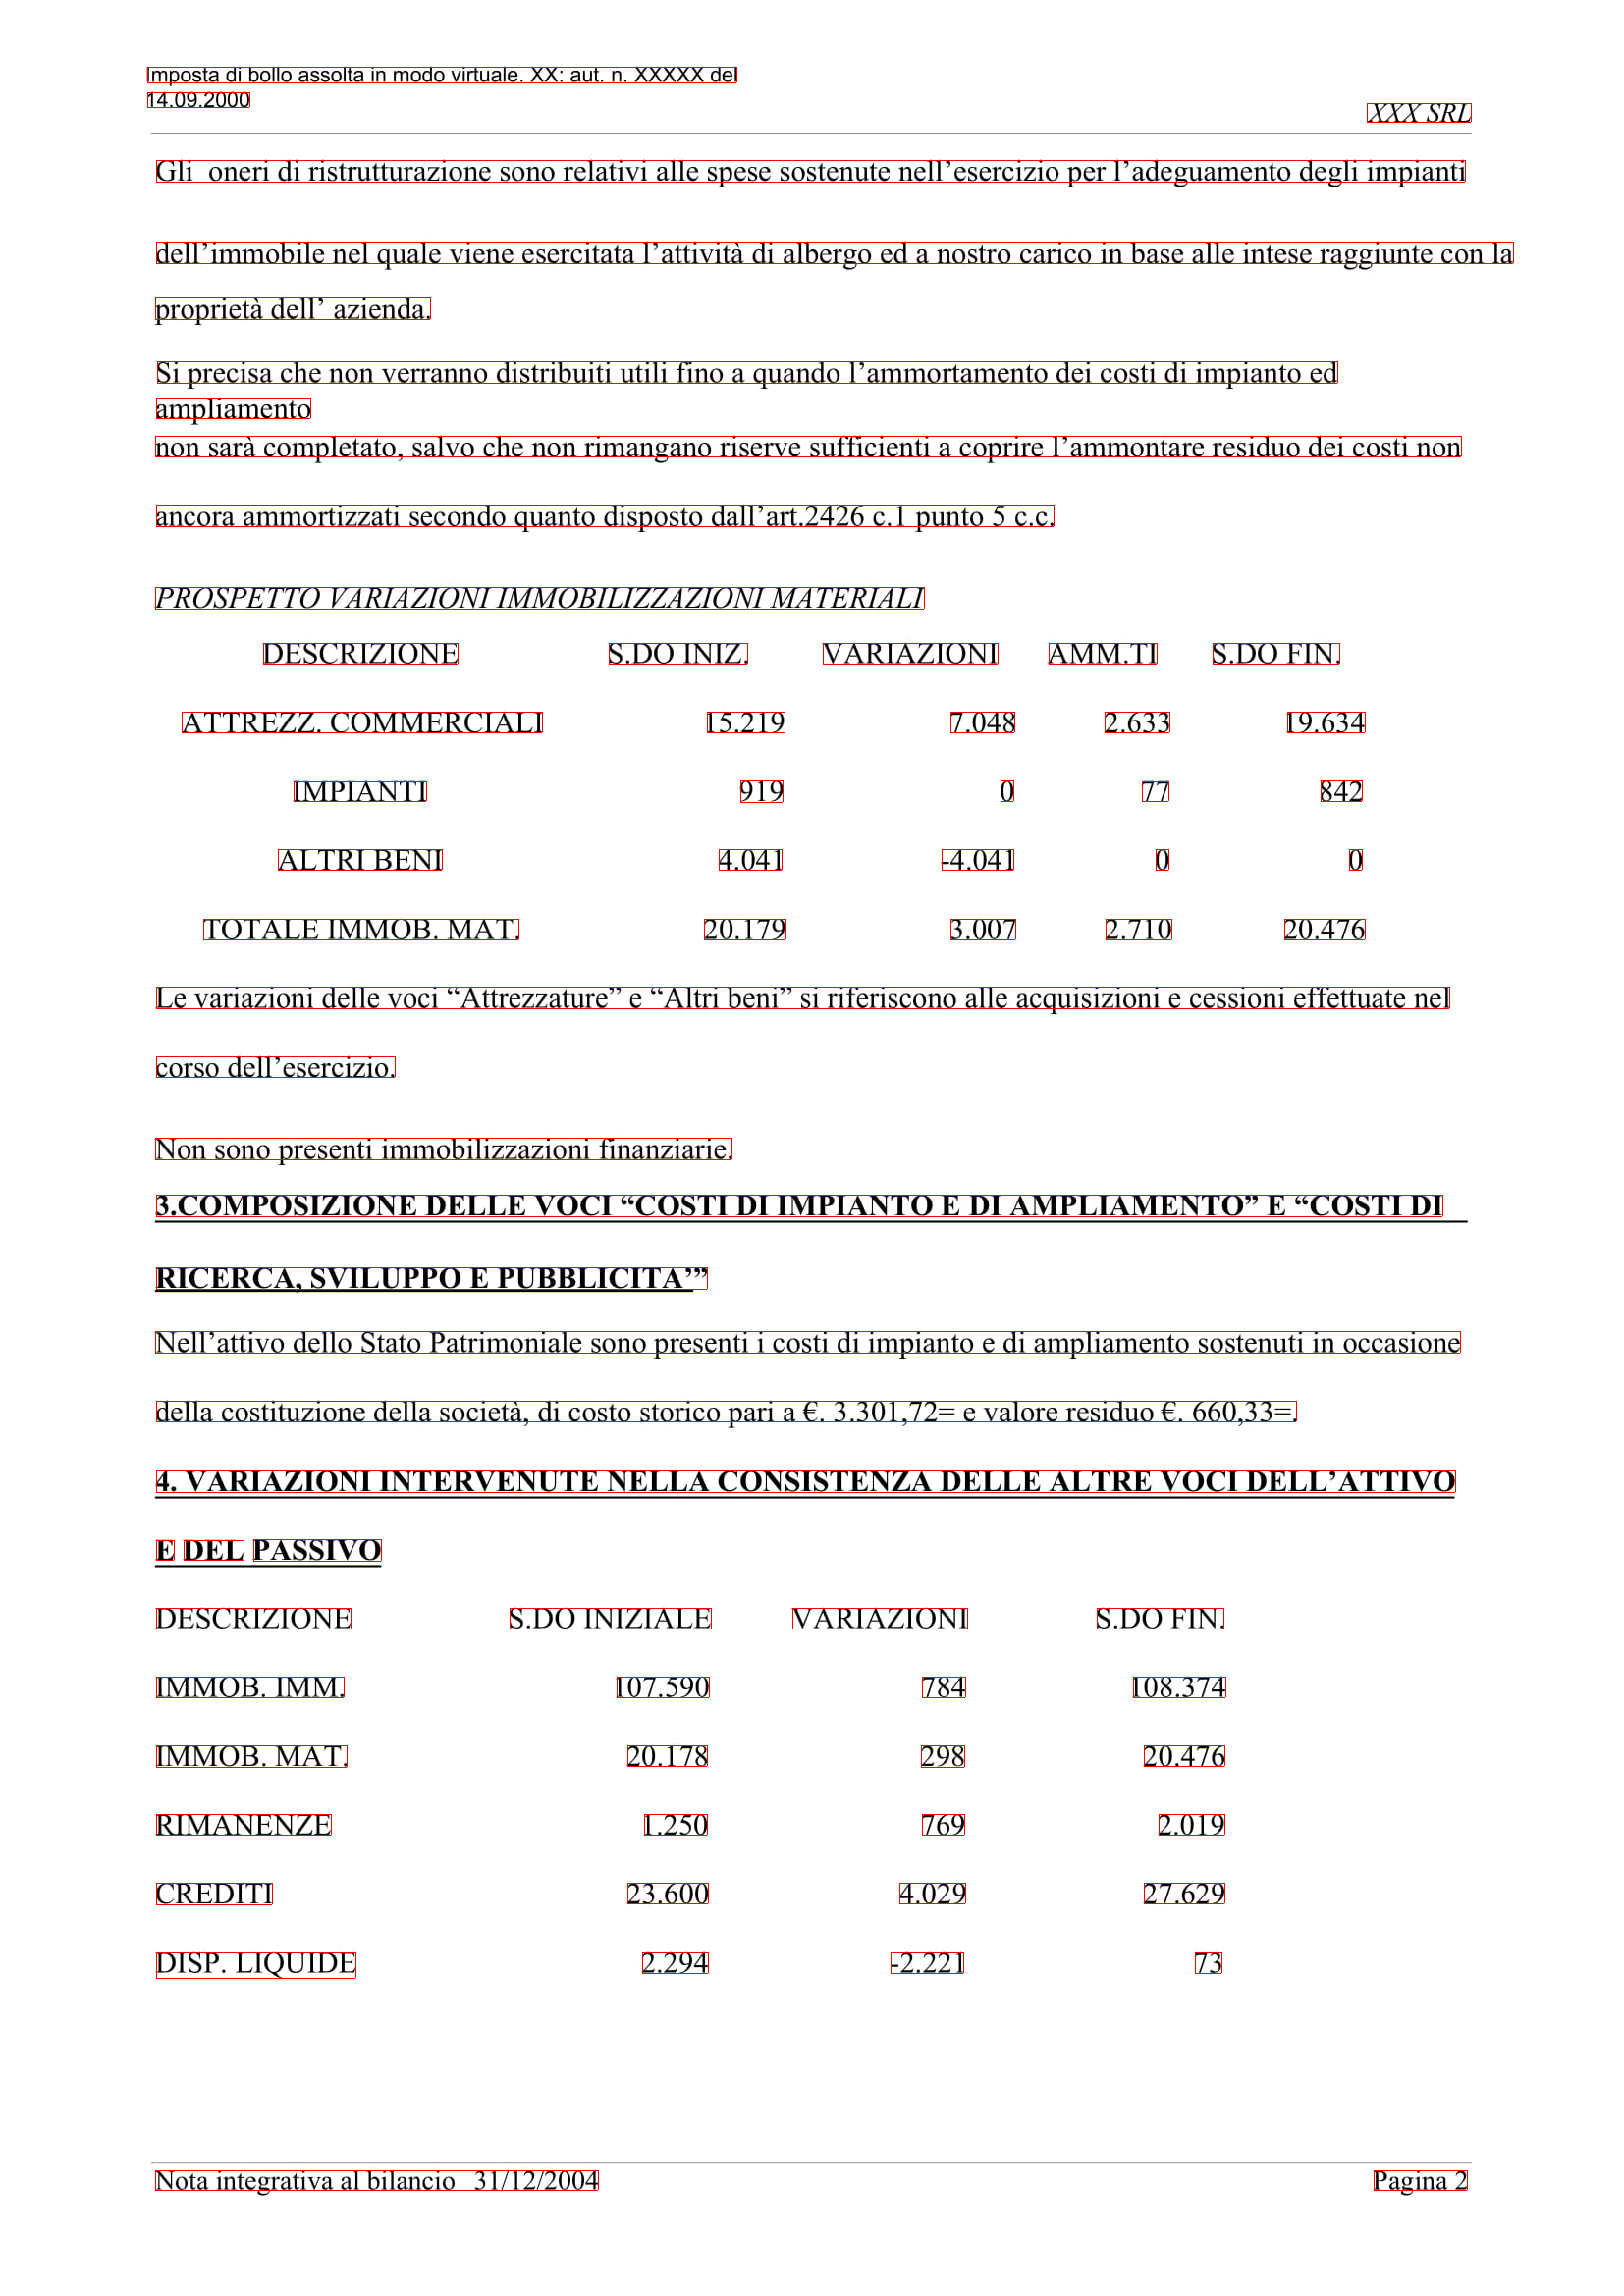
\includegraphics[width=\linewidth]{img/implementation/implem3.png}
\caption{The results of segmentation of each textline into columns.}
\label{fig:implem3}
\end{subfigure}
\qquad
\begin{subfigure}{0.45\textwidth}
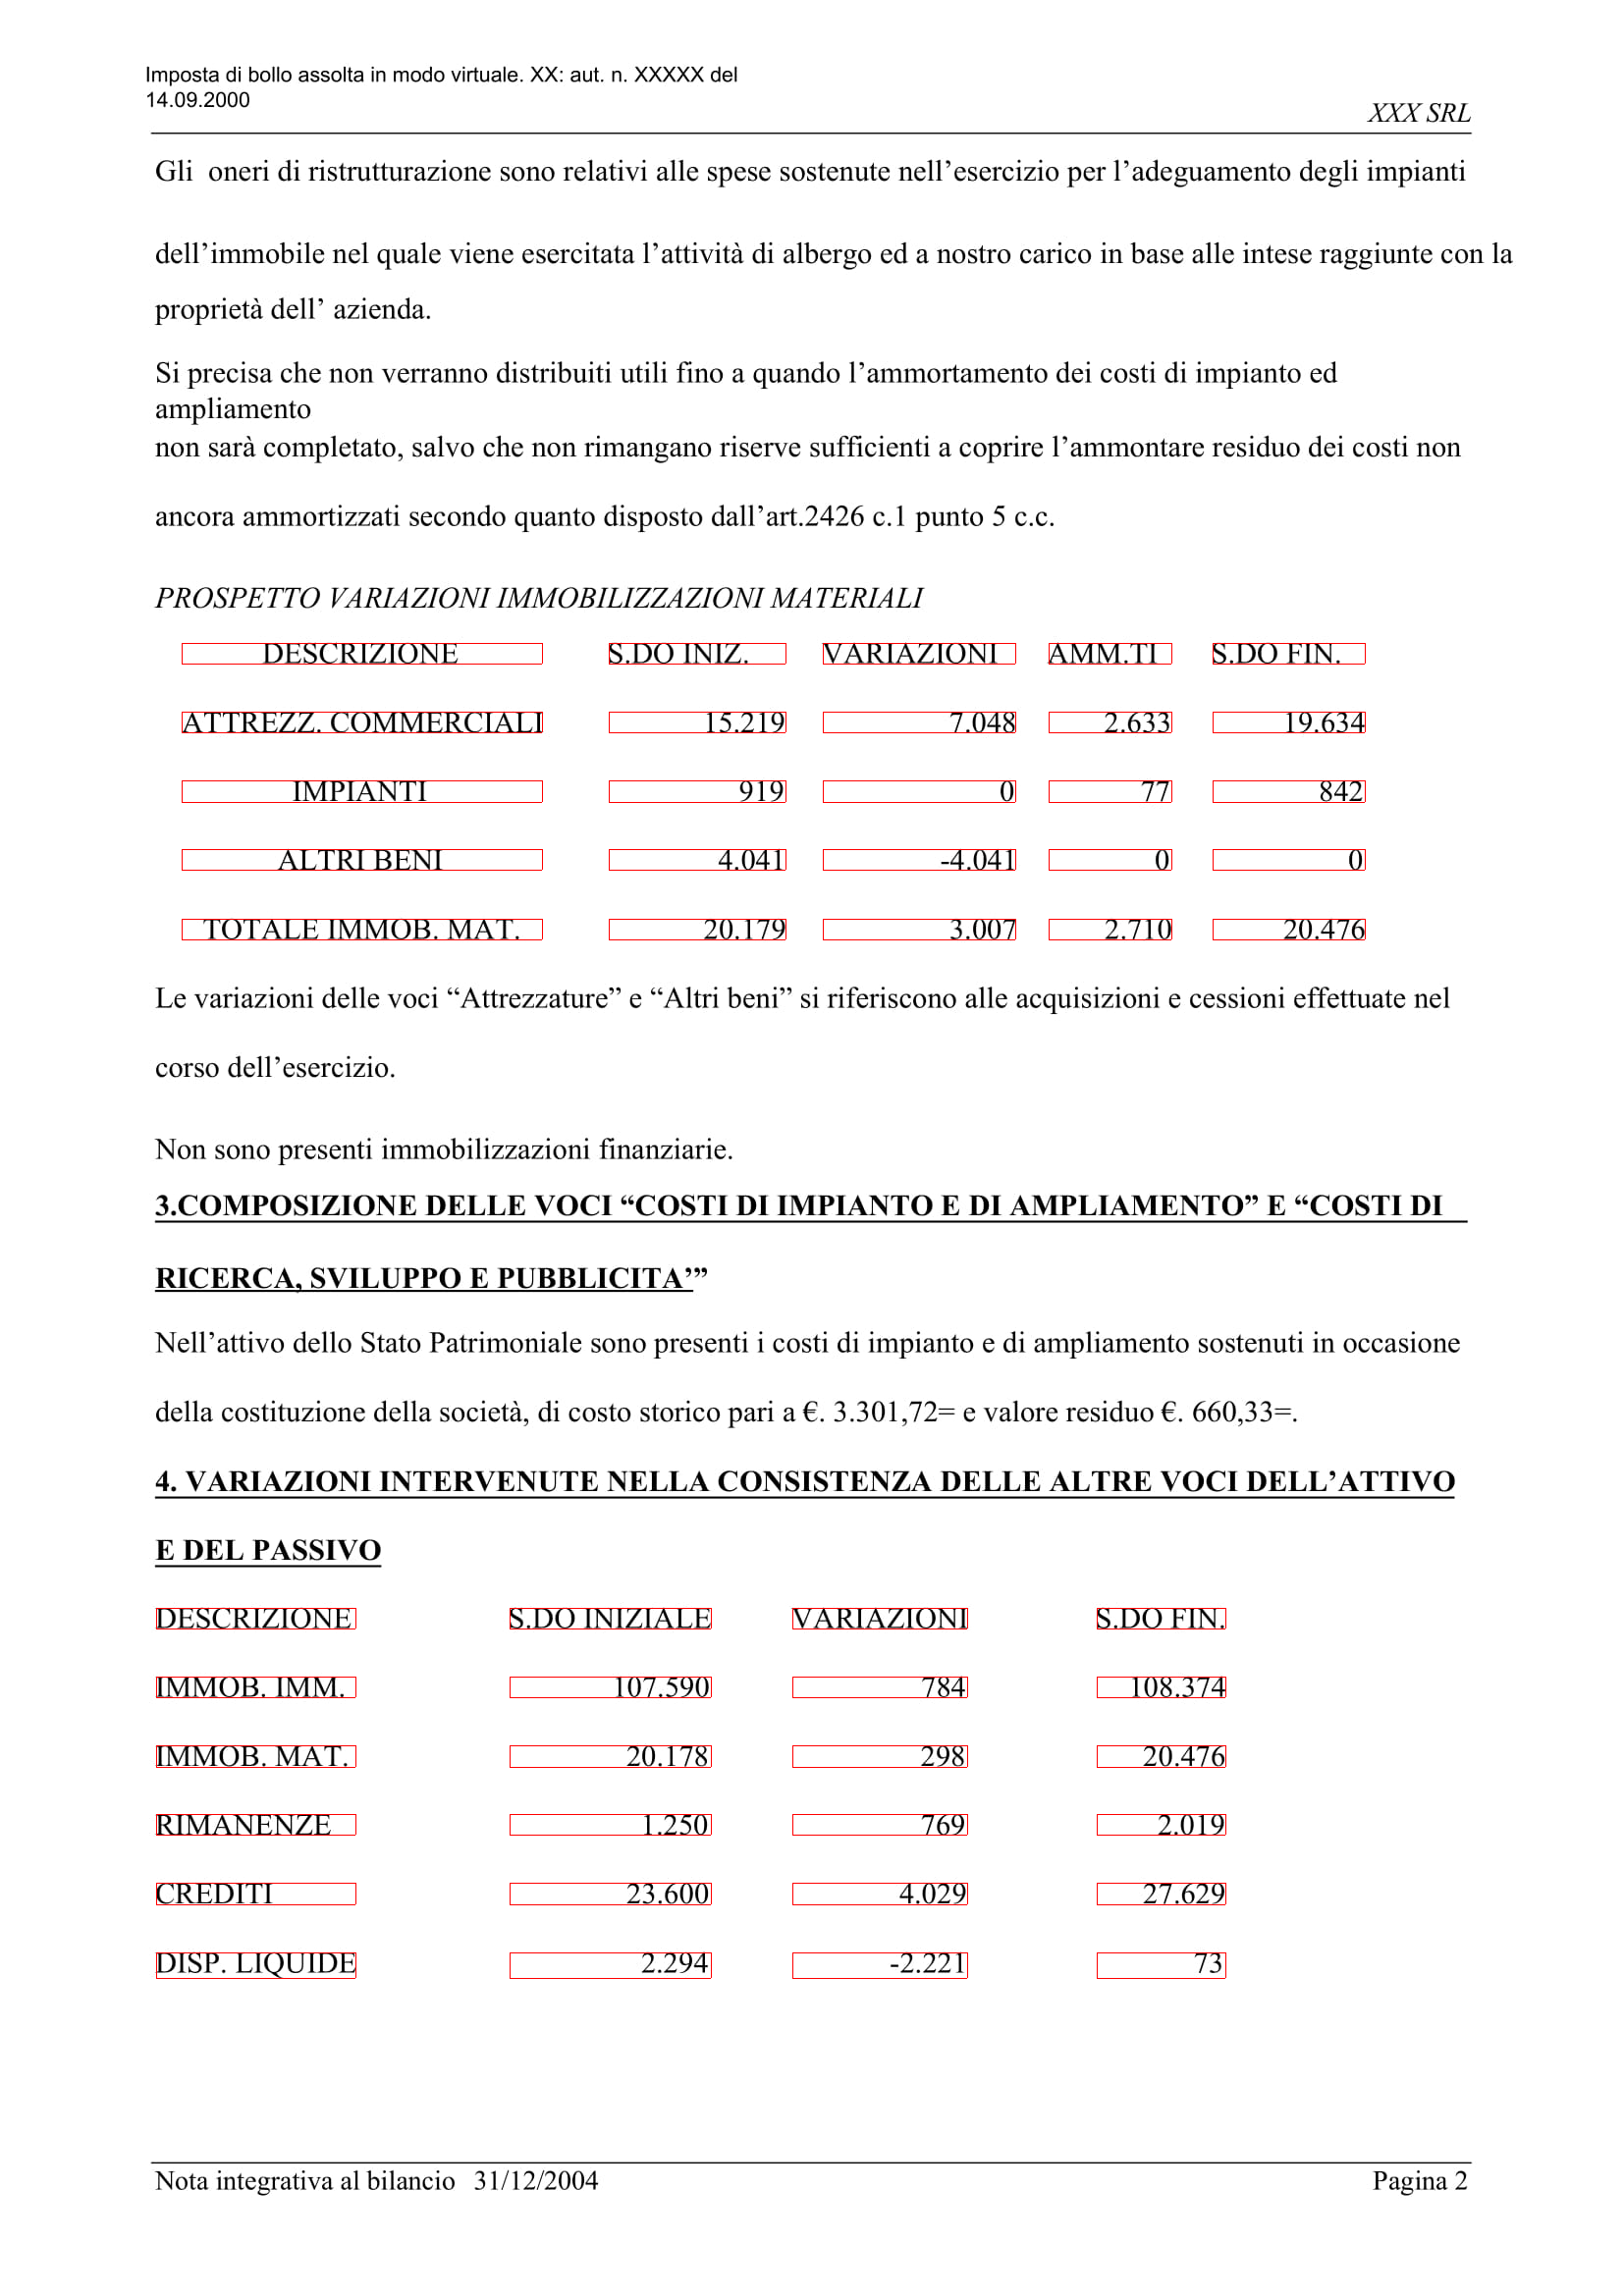
\includegraphics[width=\linewidth]{img/implementation/implem4.png}
\caption{Result of our algorithm: individual bordered cells that represent tables.}
\label{fig:implem4}
\end{subfigure}
\caption{The process of table recognition.}
\label{fig:implemTableRecogniton}
\end{figure}
